\documentclass[12pt]{article}
\usepackage{tikz}
\usepackage{amsmath}
% Underlining package
\usepackage{ulem}
\usetikzlibrary{calc}
\usetikzlibrary{angles,quotes}
\usepackage[a4paper, portrait, margin=1cm]{geometry}
\usepackage{fancyhdr}

\newcommand{\HeadingAnswers}{%
\section*{\Large Name: \underline{\hspace{8cm}} \hfill Date: \underline{\hspace{3cm}}}%
\vspace{-3mm}\par
\textbf{Area Rectangles: Answers}\vspace{1pt}\hrule
}

% raise footer with page number; no header
\fancypagestyle{myfancypagestyle}{
  \fancyhf{}% clear all header and footer fields
  \renewcommand{\headrulewidth}{0pt} % no rule under header
  \fancyfoot[C] {\thepage} \setlength{\footskip}{14.5pt} % raise page number allowed min 14.5pt
}
\pagestyle{myfancypagestyle}  % apply myfancypagestyle

\newcounter{minipagecount}

\begin{document}
\HeadingAnswers
\vspace{8mm}

\begin{minipage}{0.55\textwidth}
  \refstepcounter{minipagecount}
  \noindent{(\theminipagecount)}\quad
  \begin{tikzpicture}[scale=1.1, baseline=(current bounding box.north)]
    \begin{scope}[rotate=0]
        % Draw square
        \draw (0,0) coordinate (K) --
              ++(2.596,0) coordinate (L) --
              ++(0,1.854) coordinate (M) --
              ++(-2.596,0) coordinate (N) -- cycle;

        % Right angle markers
        \foreach \p/\q/\r in {N/K/L,K/L/M,M/N/K,N/K/L} {
            \pic [draw, -, angle radius=0.2cm] {right angle=\p--\q--\r};
        }

        % Vertex LABELS
        \foreach \p/\l in {K/below left,L/below right,M/above right,N/above left} {
            \node[\l] at (\p) {\p};
        }

        % Dotted arrows shifted away from edges
        % Horizontal side (A-B), shifted down
        \draw[<->, dotted]
            ($(K) + (0,-0.2cm)$) -- ($(L) + (0,-0.2cm)$)
            node[midway,below, xshift=2mm] {7\,cm};

        % Vertical side (B-C), shifted right
        \draw[<->, dotted]
            ($(L) + (0.2cm,0)$) -- ($(M) + (0.2cm,0)$)
            node[midway,right] {5\,cm};
    \end{scope}
\end{tikzpicture}
\end{minipage}%
\hfill
\begin{minipage}{.4\textwidth}
  \begin{align*}
  \text{Area} &= lw \\
  \text{Area} &= 7 \,\text{cm} \times 5 \,\text{cm} \\
  \text{Area} &= 35 \,\text{cm}^2
  \end{align*}
\end{minipage}
\par\vspace{1cm}\begin{minipage}{0.55\textwidth}
  \refstepcounter{minipagecount}
  \noindent{(\theminipagecount)}\quad
  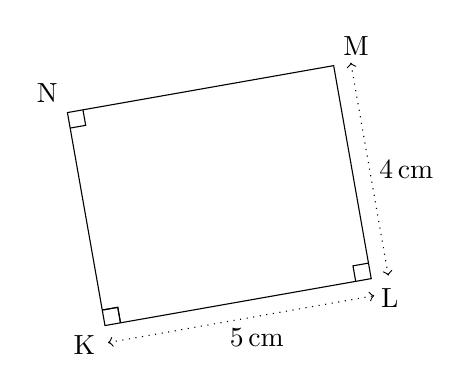
\begin{tikzpicture}[scale=1.1, baseline=(current bounding box.north)]
    \begin{scope}[rotate=10]
        % Draw square
        \draw (0,0) coordinate (K) --
              ++(3.121,0) coordinate (L) --
              ++(0,2.497) coordinate (M) --
              ++(-3.121,0) coordinate (N) -- cycle;

        % Right angle markers
        \foreach \p/\q/\r in {N/K/L,K/L/M,M/N/K,N/K/L} {
            \pic [draw, -, angle radius=0.2cm] {right angle=\p--\q--\r};
        }

        % Vertex LABELS
        \foreach \p/\l in {K/below left,L/below right,M/above right,N/above left} {
            \node[\l] at (\p) {\p};
        }

        % Dotted arrows shifted away from edges
        % Horizontal side (A-B), shifted down
        \draw[<->, dotted]
            ($(K) + (0,-0.2cm)$) -- ($(L) + (0,-0.2cm)$)
            node[midway,below, xshift=2mm] {5\,cm};

        % Vertical side (B-C), shifted right
        \draw[<->, dotted]
            ($(L) + (0.2cm,0)$) -- ($(M) + (0.2cm,0)$)
            node[midway,right] {4\,cm};
    \end{scope}
\end{tikzpicture}
\end{minipage}%
\hfill
\begin{minipage}{.4\textwidth}
  \begin{align*}
  \text{Area} &= lw \\
  \text{Area} &= 5 \,\text{cm} \times 4 \,\text{cm} \\
  \text{Area} &= 20 \,\text{cm}^2
  \end{align*}
\end{minipage}
\par\vspace{1cm}\begin{minipage}{0.55\textwidth}
  \refstepcounter{minipagecount}
  \noindent{(\theminipagecount)}\quad
  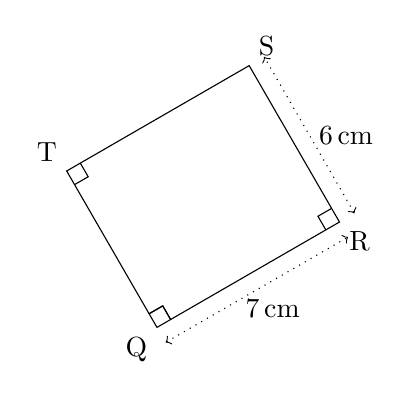
\begin{tikzpicture}[scale=1.1, baseline=(current bounding box.north)]
    \begin{scope}[rotate=30]
        % Draw square
        \draw (0,0) coordinate (Q) --
              ++(2.433,0) coordinate (R) --
              ++(0,2.085) coordinate (S) --
              ++(-2.433,0) coordinate (T) -- cycle;

        % Right angle markers
        \foreach \p/\q/\r in {T/Q/R,Q/R/S,S/T/Q,T/Q/R} {
            \pic [draw, -, angle radius=0.2cm] {right angle=\p--\q--\r};
        }

        % Vertex LABELS
        \foreach \p/\l in {Q/below left,R/below right,S/above right,T/above left} {
            \node[\l] at (\p) {\p};
        }

        % Dotted arrows shifted away from edges
        % Horizontal side (A-B), shifted down
        \draw[<->, dotted]
            ($(Q) + (0,-0.2cm)$) -- ($(R) + (0,-0.2cm)$)
            node[midway,below, xshift=2mm] {7\,cm};

        % Vertical side (B-C), shifted right
        \draw[<->, dotted]
            ($(R) + (0.2cm,0)$) -- ($(S) + (0.2cm,0)$)
            node[midway,right] {6\,cm};
    \end{scope}
\end{tikzpicture}
\end{minipage}%
\hfill
\begin{minipage}{.4\textwidth}
  \begin{align*}
  \text{Area} &= lw \\
  \text{Area} &= 7 \,\text{cm} \times 6 \,\text{cm} \\
  \text{Area} &= 42 \,\text{cm}^2
  \end{align*}
\end{minipage}
\par\vspace{1cm}\begin{minipage}{0.55\textwidth}
  \refstepcounter{minipagecount}
  \noindent{(\theminipagecount)}\quad
  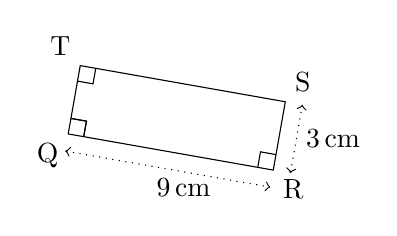
\begin{tikzpicture}[scale=1.1, baseline=(current bounding box.north)]
    \begin{scope}[rotate=-10]
        % Draw square
        \draw (0,0) coordinate (Q) --
              ++(2.404,0) coordinate (R) --
              ++(0,0.801) coordinate (S) --
              ++(-2.404,0) coordinate (T) -- cycle;

        % Right angle markers
        \foreach \p/\q/\r in {T/Q/R,Q/R/S,S/T/Q,T/Q/R} {
            \pic [draw, -, angle radius=0.2cm] {right angle=\p--\q--\r};
        }

        % Vertex LABELS
        \foreach \p/\l in {Q/below left,R/below right,S/above right,T/above left} {
            \node[\l] at (\p) {\p};
        }

        % Dotted arrows shifted away from edges
        % Horizontal side (A-B), shifted down
        \draw[<->, dotted]
            ($(Q) + (0,-0.2cm)$) -- ($(R) + (0,-0.2cm)$)
            node[midway,below, xshift=2mm] {9\,cm};

        % Vertical side (B-C), shifted right
        \draw[<->, dotted]
            ($(R) + (0.2cm,0)$) -- ($(S) + (0.2cm,0)$)
            node[midway,right] {3\,cm};
    \end{scope}
\end{tikzpicture}
\end{minipage}%
\hfill
\begin{minipage}{.4\textwidth}
  \begin{align*}
  \text{Area} &= lw \\
  \text{Area} &= 9 \,\text{cm} \times 3 \,\text{cm} \\
  \text{Area} &= 27 \,\text{cm}^2
  \end{align*}
\end{minipage}
\par\vspace{1cm}\begin{minipage}{0.55\textwidth}
  \refstepcounter{minipagecount}
  \noindent{(\theminipagecount)}\quad
  \begin{tikzpicture}[scale=1.1, baseline=(current bounding box.north)]
    \begin{scope}[rotate=0]
        % Draw square
        \draw (0,0) coordinate (K) --
              ++(3.151,0) coordinate (L) --
              ++(0,2.363) coordinate (M) --
              ++(-3.151,0) coordinate (N) -- cycle;

        % Right angle markers
        \foreach \p/\q/\r in {N/K/L,K/L/M,M/N/K,N/K/L} {
            \pic [draw, -, angle radius=0.2cm] {right angle=\p--\q--\r};
        }

        % Vertex LABELS
        \foreach \p/\l in {K/below left,L/below right,M/above right,N/above left} {
            \node[\l] at (\p) {\p};
        }

        % Dotted arrows shifted away from edges
        % Horizontal side (A-B), shifted down
        \draw[<->, dotted]
            ($(K) + (0,-0.2cm)$) -- ($(L) + (0,-0.2cm)$)
            node[midway,below, xshift=2mm] {8\,cm};

        % Vertical side (B-C), shifted right
        \draw[<->, dotted]
            ($(L) + (0.2cm,0)$) -- ($(M) + (0.2cm,0)$)
            node[midway,right] {6\,cm};
    \end{scope}
\end{tikzpicture}
\end{minipage}%
\hfill
\begin{minipage}{.4\textwidth}
  \begin{align*}
  \text{Area} &= lw \\
  \text{Area} &= 8 \,\text{cm} \times 6 \,\text{cm} \\
  \text{Area} &= 48 \,\text{cm}^2
  \end{align*}
\end{minipage}
\par\vspace{1cm}\begin{minipage}{0.55\textwidth}
  \refstepcounter{minipagecount}
  \noindent{(\theminipagecount)}\quad
  \begin{tikzpicture}[scale=1.1, baseline=(current bounding box.north)]
    \begin{scope}[rotate=-45]
        % Draw square
        \draw (0,0) coordinate (A) --
              ++(3.35,0) coordinate (B) --
              ++(0,1.861) coordinate (C) --
              ++(-3.35,0) coordinate (D) -- cycle;

        % Right angle markers
        \foreach \p/\q/\r in {D/A/B,A/B/C,C/D/A,D/A/B} {
            \pic [draw, -, angle radius=0.2cm] {right angle=\p--\q--\r};
        }

        % Vertex LABELS
        \foreach \p/\l in {A/below left,B/below right,C/above right,D/above left} {
            \node[\l] at (\p) {\p};
        }

        % Dotted arrows shifted away from edges
        % Horizontal side (A-B), shifted down
        \draw[<->, dotted]
            ($(A) + (0,-0.2cm)$) -- ($(B) + (0,-0.2cm)$)
            node[midway,below, xshift=2mm] {9\,cm};

        % Vertical side (B-C), shifted right
        \draw[<->, dotted]
            ($(B) + (0.2cm,0)$) -- ($(C) + (0.2cm,0)$)
            node[midway,right] {5\,cm};
    \end{scope}
\end{tikzpicture}
\end{minipage}%
\hfill
\begin{minipage}{.4\textwidth}
  \begin{align*}
  \text{Area} &= lw \\
  \text{Area} &= 9 \,\text{cm} \times 5 \,\text{cm} \\
  \text{Area} &= 45 \,\text{cm}^2
  \end{align*}
\end{minipage}
\par\vspace{1cm}\begin{minipage}{0.55\textwidth}
  \refstepcounter{minipagecount}
  \noindent{(\theminipagecount)}\quad
  \begin{tikzpicture}[scale=1.1, baseline=(current bounding box.north)]
    \begin{scope}[rotate=0]
        % Draw square
        \draw (0,0) coordinate (E) --
              ++(2.593,0) coordinate (F) --
              ++(0,2.305) coordinate (G) --
              ++(-2.593,0) coordinate (H) -- cycle;

        % Right angle markers
        \foreach \p/\q/\r in {H/E/F,E/F/G,G/H/E,H/E/F} {
            \pic [draw, -, angle radius=0.2cm] {right angle=\p--\q--\r};
        }

        % Vertex LABELS
        \foreach \p/\l in {E/below left,F/below right,G/above right,H/above left} {
            \node[\l] at (\p) {\p};
        }

        % Dotted arrows shifted away from edges
        % Horizontal side (A-B), shifted down
        \draw[<->, dotted]
            ($(E) + (0,-0.2cm)$) -- ($(F) + (0,-0.2cm)$)
            node[midway,below, xshift=2mm] {9\,cm};

        % Vertical side (B-C), shifted right
        \draw[<->, dotted]
            ($(F) + (0.2cm,0)$) -- ($(G) + (0.2cm,0)$)
            node[midway,right] {8\,cm};
    \end{scope}
\end{tikzpicture}
\end{minipage}%
\hfill
\begin{minipage}{.4\textwidth}
  \begin{align*}
  \text{Area} &= lw \\
  \text{Area} &= 9 \,\text{cm} \times 8 \,\text{cm} \\
  \text{Area} &= 72 \,\text{cm}^2
  \end{align*}
\end{minipage}
\par\vspace{1cm}\begin{minipage}{0.55\textwidth}
  \refstepcounter{minipagecount}
  \noindent{(\theminipagecount)}\quad
  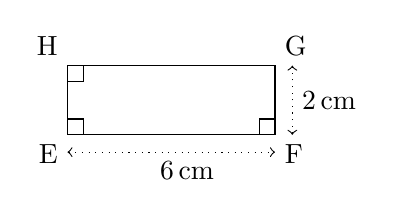
\begin{tikzpicture}[scale=1.1, baseline=(current bounding box.north)]
    \begin{scope}[rotate=0]
        % Draw square
        \draw (0,0) coordinate (E) --
              ++(2.396,0) coordinate (F) --
              ++(0,0.799) coordinate (G) --
              ++(-2.396,0) coordinate (H) -- cycle;

        % Right angle markers
        \foreach \p/\q/\r in {H/E/F,E/F/G,G/H/E,H/E/F} {
            \pic [draw, -, angle radius=0.2cm] {right angle=\p--\q--\r};
        }

        % Vertex LABELS
        \foreach \p/\l in {E/below left,F/below right,G/above right,H/above left} {
            \node[\l] at (\p) {\p};
        }

        % Dotted arrows shifted away from edges
        % Horizontal side (A-B), shifted down
        \draw[<->, dotted]
            ($(E) + (0,-0.2cm)$) -- ($(F) + (0,-0.2cm)$)
            node[midway,below, xshift=2mm] {6\,cm};

        % Vertical side (B-C), shifted right
        \draw[<->, dotted]
            ($(F) + (0.2cm,0)$) -- ($(G) + (0.2cm,0)$)
            node[midway,right] {2\,cm};
    \end{scope}
\end{tikzpicture}
\end{minipage}%
\hfill
\begin{minipage}{.4\textwidth}
  \begin{align*}
  \text{Area} &= lw \\
  \text{Area} &= 6 \,\text{cm} \times 2 \,\text{cm} \\
  \text{Area} &= 12 \,\text{cm}^2
  \end{align*}
\end{minipage}
\par\vspace{1cm}\begin{minipage}{0.55\textwidth}
  \refstepcounter{minipagecount}
  \noindent{(\theminipagecount)}\quad
  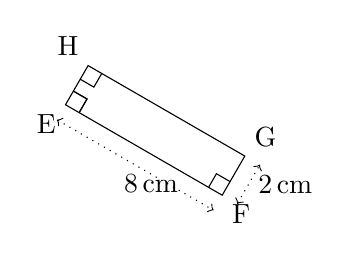
\begin{tikzpicture}[scale=1.1, baseline=(current bounding box.north)]
    \begin{scope}[rotate=-30]
        % Draw square
        \draw (0,0) coordinate (E) --
              ++(2.089,0) coordinate (F) --
              ++(0,0.522) coordinate (G) --
              ++(-2.089,0) coordinate (H) -- cycle;

        % Right angle markers
        \foreach \p/\q/\r in {H/E/F,E/F/G,G/H/E,H/E/F} {
            \pic [draw, -, angle radius=0.2cm] {right angle=\p--\q--\r};
        }

        % Vertex LABELS
        \foreach \p/\l in {E/below left,F/below right,G/above right,H/above left} {
            \node[\l] at (\p) {\p};
        }

        % Dotted arrows shifted away from edges
        % Horizontal side (A-B), shifted down
        \draw[<->, dotted]
            ($(E) + (0,-0.2cm)$) -- ($(F) + (0,-0.2cm)$)
            node[midway,below, xshift=2mm] {8\,cm};

        % Vertical side (B-C), shifted right
        \draw[<->, dotted]
            ($(F) + (0.2cm,0)$) -- ($(G) + (0.2cm,0)$)
            node[midway,right] {2\,cm};
    \end{scope}
\end{tikzpicture}
\end{minipage}%
\hfill
\begin{minipage}{.4\textwidth}
  \begin{align*}
  \text{Area} &= lw \\
  \text{Area} &= 8 \,\text{cm} \times 2 \,\text{cm} \\
  \text{Area} &= 16 \,\text{cm}^2
  \end{align*}
\end{minipage}
\par\vspace{1cm}\begin{minipage}{0.55\textwidth}
  \refstepcounter{minipagecount}
  \noindent{(\theminipagecount)}\quad
  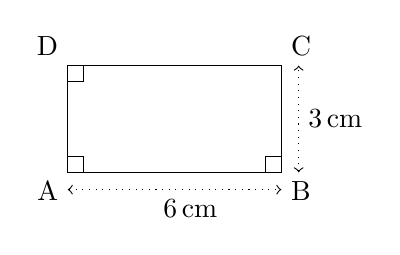
\begin{tikzpicture}[scale=1.1, baseline=(current bounding box.north)]
    \begin{scope}[rotate=0]
        % Draw square
        \draw (0,0) coordinate (A) --
              ++(2.465,0) coordinate (B) --
              ++(0,1.232) coordinate (C) --
              ++(-2.465,0) coordinate (D) -- cycle;

        % Right angle markers
        \foreach \p/\q/\r in {D/A/B,A/B/C,C/D/A,D/A/B} {
            \pic [draw, -, angle radius=0.2cm] {right angle=\p--\q--\r};
        }

        % Vertex LABELS
        \foreach \p/\l in {A/below left,B/below right,C/above right,D/above left} {
            \node[\l] at (\p) {\p};
        }

        % Dotted arrows shifted away from edges
        % Horizontal side (A-B), shifted down
        \draw[<->, dotted]
            ($(A) + (0,-0.2cm)$) -- ($(B) + (0,-0.2cm)$)
            node[midway,below, xshift=2mm] {6\,cm};

        % Vertical side (B-C), shifted right
        \draw[<->, dotted]
            ($(B) + (0.2cm,0)$) -- ($(C) + (0.2cm,0)$)
            node[midway,right] {3\,cm};
    \end{scope}
\end{tikzpicture}
\end{minipage}%
\hfill
\begin{minipage}{.4\textwidth}
  \begin{align*}
  \text{Area} &= lw \\
  \text{Area} &= 6 \,\text{cm} \times 3 \,\text{cm} \\
  \text{Area} &= 18 \,\text{cm}^2
  \end{align*}
\end{minipage}
\par\vspace{1cm}\begin{minipage}{0.55\textwidth}
  \refstepcounter{minipagecount}
  \noindent{(\theminipagecount)}\quad
  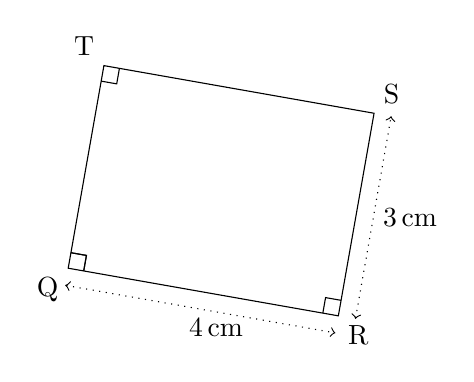
\begin{tikzpicture}[scale=1.1, baseline=(current bounding box.north)]
    \begin{scope}[rotate=-10]
        % Draw square
        \draw (0,0) coordinate (Q) --
              ++(3.167,0) coordinate (R) --
              ++(0,2.375) coordinate (S) --
              ++(-3.167,0) coordinate (T) -- cycle;

        % Right angle markers
        \foreach \p/\q/\r in {T/Q/R,Q/R/S,S/T/Q,T/Q/R} {
            \pic [draw, -, angle radius=0.2cm] {right angle=\p--\q--\r};
        }

        % Vertex LABELS
        \foreach \p/\l in {Q/below left,R/below right,S/above right,T/above left} {
            \node[\l] at (\p) {\p};
        }

        % Dotted arrows shifted away from edges
        % Horizontal side (A-B), shifted down
        \draw[<->, dotted]
            ($(Q) + (0,-0.2cm)$) -- ($(R) + (0,-0.2cm)$)
            node[midway,below, xshift=2mm] {4\,cm};

        % Vertical side (B-C), shifted right
        \draw[<->, dotted]
            ($(R) + (0.2cm,0)$) -- ($(S) + (0.2cm,0)$)
            node[midway,right] {3\,cm};
    \end{scope}
\end{tikzpicture}
\end{minipage}%
\hfill
\begin{minipage}{.4\textwidth}
  \begin{align*}
  \text{Area} &= lw \\
  \text{Area} &= 4 \,\text{cm} \times 3 \,\text{cm} \\
  \text{Area} &= 12 \,\text{cm}^2
  \end{align*}
\end{minipage}
\par\vspace{1cm}\begin{minipage}{0.55\textwidth}
  \refstepcounter{minipagecount}
  \noindent{(\theminipagecount)}\quad
  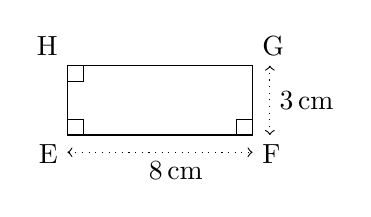
\begin{tikzpicture}[scale=1.1, baseline=(current bounding box.north)]
    \begin{scope}[rotate=0]
        % Draw square
        \draw (0,0) coordinate (E) --
              ++(2.137,0) coordinate (F) --
              ++(0,0.801) coordinate (G) --
              ++(-2.137,0) coordinate (H) -- cycle;

        % Right angle markers
        \foreach \p/\q/\r in {H/E/F,E/F/G,G/H/E,H/E/F} {
            \pic [draw, -, angle radius=0.2cm] {right angle=\p--\q--\r};
        }

        % Vertex LABELS
        \foreach \p/\l in {E/below left,F/below right,G/above right,H/above left} {
            \node[\l] at (\p) {\p};
        }

        % Dotted arrows shifted away from edges
        % Horizontal side (A-B), shifted down
        \draw[<->, dotted]
            ($(E) + (0,-0.2cm)$) -- ($(F) + (0,-0.2cm)$)
            node[midway,below, xshift=2mm] {8\,cm};

        % Vertical side (B-C), shifted right
        \draw[<->, dotted]
            ($(F) + (0.2cm,0)$) -- ($(G) + (0.2cm,0)$)
            node[midway,right] {3\,cm};
    \end{scope}
\end{tikzpicture}
\end{minipage}%
\hfill
\begin{minipage}{.4\textwidth}
  \begin{align*}
  \text{Area} &= lw \\
  \text{Area} &= 8 \,\text{cm} \times 3 \,\text{cm} \\
  \text{Area} &= 24 \,\text{cm}^2
  \end{align*}
\end{minipage}
\par\vspace{1cm}\begin{minipage}{0.55\textwidth}
  \refstepcounter{minipagecount}
  \noindent{(\theminipagecount)}\quad
  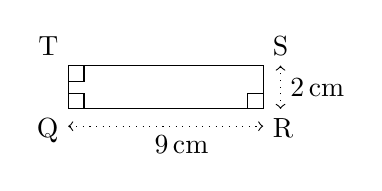
\begin{tikzpicture}[scale=1.1, baseline=(current bounding box.north)]
    \begin{scope}[rotate=0]
        % Draw square
        \draw (0,0) coordinate (Q) --
              ++(2.251,0) coordinate (R) --
              ++(0,0.5) coordinate (S) --
              ++(-2.251,0) coordinate (T) -- cycle;

        % Right angle markers
        \foreach \p/\q/\r in {T/Q/R,Q/R/S,S/T/Q,T/Q/R} {
            \pic [draw, -, angle radius=0.2cm] {right angle=\p--\q--\r};
        }

        % Vertex LABELS
        \foreach \p/\l in {Q/below left,R/below right,S/above right,T/above left} {
            \node[\l] at (\p) {\p};
        }

        % Dotted arrows shifted away from edges
        % Horizontal side (A-B), shifted down
        \draw[<->, dotted]
            ($(Q) + (0,-0.2cm)$) -- ($(R) + (0,-0.2cm)$)
            node[midway,below, xshift=2mm] {9\,cm};

        % Vertical side (B-C), shifted right
        \draw[<->, dotted]
            ($(R) + (0.2cm,0)$) -- ($(S) + (0.2cm,0)$)
            node[midway,right] {2\,cm};
    \end{scope}
\end{tikzpicture}
\end{minipage}%
\hfill
\begin{minipage}{.4\textwidth}
  \begin{align*}
  \text{Area} &= lw \\
  \text{Area} &= 9 \,\text{cm} \times 2 \,\text{cm} \\
  \text{Area} &= 18 \,\text{cm}^2
  \end{align*}
\end{minipage}
\par\vspace{1cm}\begin{minipage}{0.55\textwidth}
  \refstepcounter{minipagecount}
  \noindent{(\theminipagecount)}\quad
  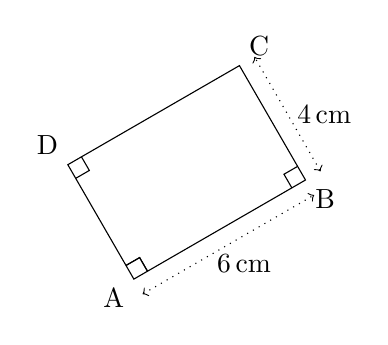
\begin{tikzpicture}[scale=1.1, baseline=(current bounding box.north)]
    \begin{scope}[rotate=30]
        % Draw square
        \draw (0,0) coordinate (A) --
              ++(2.288,0) coordinate (B) --
              ++(0,1.525) coordinate (C) --
              ++(-2.288,0) coordinate (D) -- cycle;

        % Right angle markers
        \foreach \p/\q/\r in {D/A/B,A/B/C,C/D/A,D/A/B} {
            \pic [draw, -, angle radius=0.2cm] {right angle=\p--\q--\r};
        }

        % Vertex LABELS
        \foreach \p/\l in {A/below left,B/below right,C/above right,D/above left} {
            \node[\l] at (\p) {\p};
        }

        % Dotted arrows shifted away from edges
        % Horizontal side (A-B), shifted down
        \draw[<->, dotted]
            ($(A) + (0,-0.2cm)$) -- ($(B) + (0,-0.2cm)$)
            node[midway,below, xshift=2mm] {6\,cm};

        % Vertical side (B-C), shifted right
        \draw[<->, dotted]
            ($(B) + (0.2cm,0)$) -- ($(C) + (0.2cm,0)$)
            node[midway,right] {4\,cm};
    \end{scope}
\end{tikzpicture}
\end{minipage}%
\hfill
\begin{minipage}{.4\textwidth}
  \begin{align*}
  \text{Area} &= lw \\
  \text{Area} &= 6 \,\text{cm} \times 4 \,\text{cm} \\
  \text{Area} &= 24 \,\text{cm}^2
  \end{align*}
\end{minipage}
\par\vspace{1cm}\begin{minipage}{0.55\textwidth}
  \refstepcounter{minipagecount}
  \noindent{(\theminipagecount)}\quad
  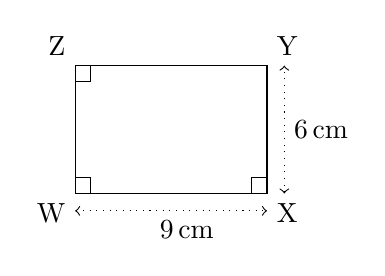
\begin{tikzpicture}[scale=1.1, baseline=(current bounding box.north)]
    \begin{scope}[rotate=0]
        % Draw square
        \draw (0,0) coordinate (W) --
              ++(2.215,0) coordinate (X) --
              ++(0,1.477) coordinate (Y) --
              ++(-2.215,0) coordinate (Z) -- cycle;

        % Right angle markers
        \foreach \p/\q/\r in {Z/W/X,W/X/Y,Y/Z/W,Z/W/X} {
            \pic [draw, -, angle radius=0.2cm] {right angle=\p--\q--\r};
        }

        % Vertex LABELS
        \foreach \p/\l in {W/below left,X/below right,Y/above right,Z/above left} {
            \node[\l] at (\p) {\p};
        }

        % Dotted arrows shifted away from edges
        % Horizontal side (A-B), shifted down
        \draw[<->, dotted]
            ($(W) + (0,-0.2cm)$) -- ($(X) + (0,-0.2cm)$)
            node[midway,below, xshift=2mm] {9\,cm};

        % Vertical side (B-C), shifted right
        \draw[<->, dotted]
            ($(X) + (0.2cm,0)$) -- ($(Y) + (0.2cm,0)$)
            node[midway,right] {6\,cm};
    \end{scope}
\end{tikzpicture}
\end{minipage}%
\hfill
\begin{minipage}{.4\textwidth}
  \begin{align*}
  \text{Area} &= lw \\
  \text{Area} &= 9 \,\text{cm} \times 6 \,\text{cm} \\
  \text{Area} &= 54 \,\text{cm}^2
  \end{align*}
\end{minipage}
\par\vspace{1cm}\begin{minipage}{0.55\textwidth}
  \refstepcounter{minipagecount}
  \noindent{(\theminipagecount)}\quad
  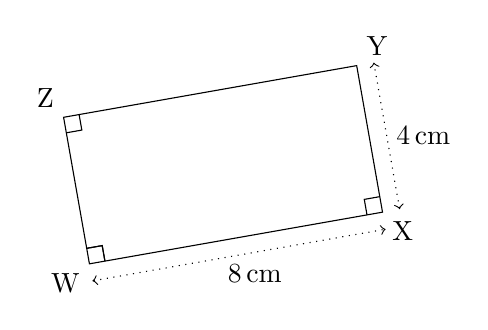
\begin{tikzpicture}[scale=1.1, baseline=(current bounding box.north)]
    \begin{scope}[rotate=10]
        % Draw square
        \draw (0,0) coordinate (W) --
              ++(3.436,0) coordinate (X) --
              ++(0,1.718) coordinate (Y) --
              ++(-3.436,0) coordinate (Z) -- cycle;

        % Right angle markers
        \foreach \p/\q/\r in {Z/W/X,W/X/Y,Y/Z/W,Z/W/X} {
            \pic [draw, -, angle radius=0.2cm] {right angle=\p--\q--\r};
        }

        % Vertex LABELS
        \foreach \p/\l in {W/below left,X/below right,Y/above right,Z/above left} {
            \node[\l] at (\p) {\p};
        }

        % Dotted arrows shifted away from edges
        % Horizontal side (A-B), shifted down
        \draw[<->, dotted]
            ($(W) + (0,-0.2cm)$) -- ($(X) + (0,-0.2cm)$)
            node[midway,below, xshift=2mm] {8\,cm};

        % Vertical side (B-C), shifted right
        \draw[<->, dotted]
            ($(X) + (0.2cm,0)$) -- ($(Y) + (0.2cm,0)$)
            node[midway,right] {4\,cm};
    \end{scope}
\end{tikzpicture}
\end{minipage}%
\hfill
\begin{minipage}{.4\textwidth}
  \begin{align*}
  \text{Area} &= lw \\
  \text{Area} &= 8 \,\text{cm} \times 4 \,\text{cm} \\
  \text{Area} &= 32 \,\text{cm}^2
  \end{align*}
\end{minipage}
\par\vspace{1cm}\begin{minipage}{0.55\textwidth}
  \refstepcounter{minipagecount}
  \noindent{(\theminipagecount)}\quad
  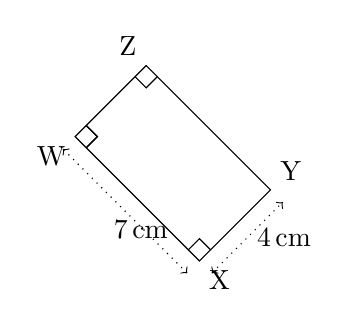
\begin{tikzpicture}[scale=1.1, baseline=(current bounding box.north)]
    \begin{scope}[rotate=-45]
        % Draw square
        \draw (0,0) coordinate (W) --
              ++(2.03,0) coordinate (X) --
              ++(0,1.16) coordinate (Y) --
              ++(-2.03,0) coordinate (Z) -- cycle;

        % Right angle markers
        \foreach \p/\q/\r in {Z/W/X,W/X/Y,Y/Z/W,Z/W/X} {
            \pic [draw, -, angle radius=0.2cm] {right angle=\p--\q--\r};
        }

        % Vertex LABELS
        \foreach \p/\l in {W/below left,X/below right,Y/above right,Z/above left} {
            \node[\l] at (\p) {\p};
        }

        % Dotted arrows shifted away from edges
        % Horizontal side (A-B), shifted down
        \draw[<->, dotted]
            ($(W) + (0,-0.2cm)$) -- ($(X) + (0,-0.2cm)$)
            node[midway,below, xshift=2mm] {7\,cm};

        % Vertical side (B-C), shifted right
        \draw[<->, dotted]
            ($(X) + (0.2cm,0)$) -- ($(Y) + (0.2cm,0)$)
            node[midway,right] {4\,cm};
    \end{scope}
\end{tikzpicture}
\end{minipage}%
\hfill
\begin{minipage}{.4\textwidth}
  \begin{align*}
  \text{Area} &= lw \\
  \text{Area} &= 7 \,\text{cm} \times 4 \,\text{cm} \\
  \text{Area} &= 28 \,\text{cm}^2
  \end{align*}
\end{minipage}
\par\vspace{1cm}\begin{minipage}{0.55\textwidth}
  \refstepcounter{minipagecount}
  \noindent{(\theminipagecount)}\quad
  \begin{tikzpicture}[scale=1.1, baseline=(current bounding box.north)]
    \begin{scope}[rotate=0]
        % Draw square
        \draw (0,0) coordinate (E) --
              ++(2.414,0) coordinate (F) --
              ++(0,2.112) coordinate (G) --
              ++(-2.414,0) coordinate (H) -- cycle;

        % Right angle markers
        \foreach \p/\q/\r in {H/E/F,E/F/G,G/H/E,H/E/F} {
            \pic [draw, -, angle radius=0.2cm] {right angle=\p--\q--\r};
        }

        % Vertex LABELS
        \foreach \p/\l in {E/below left,F/below right,G/above right,H/above left} {
            \node[\l] at (\p) {\p};
        }

        % Dotted arrows shifted away from edges
        % Horizontal side (A-B), shifted down
        \draw[<->, dotted]
            ($(E) + (0,-0.2cm)$) -- ($(F) + (0,-0.2cm)$)
            node[midway,below, xshift=2mm] {8\,cm};

        % Vertical side (B-C), shifted right
        \draw[<->, dotted]
            ($(F) + (0.2cm,0)$) -- ($(G) + (0.2cm,0)$)
            node[midway,right] {7\,cm};
    \end{scope}
\end{tikzpicture}
\end{minipage}%
\hfill
\begin{minipage}{.4\textwidth}
  \begin{align*}
  \text{Area} &= lw \\
  \text{Area} &= 8 \,\text{cm} \times 7 \,\text{cm} \\
  \text{Area} &= 56 \,\text{cm}^2
  \end{align*}
\end{minipage}
\par\vspace{1cm}\begin{minipage}{0.55\textwidth}
  \refstepcounter{minipagecount}
  \noindent{(\theminipagecount)}\quad
  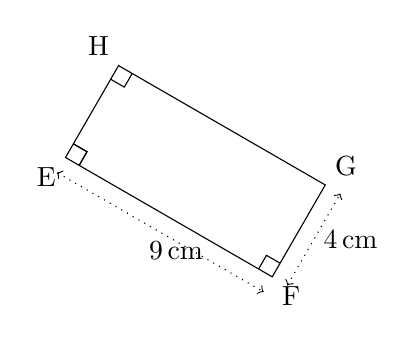
\begin{tikzpicture}[scale=1.1, baseline=(current bounding box.north)]
    \begin{scope}[rotate=-30]
        % Draw square
        \draw (0,0) coordinate (E) --
              ++(2.756,0) coordinate (F) --
              ++(0,1.225) coordinate (G) --
              ++(-2.756,0) coordinate (H) -- cycle;

        % Right angle markers
        \foreach \p/\q/\r in {H/E/F,E/F/G,G/H/E,H/E/F} {
            \pic [draw, -, angle radius=0.2cm] {right angle=\p--\q--\r};
        }

        % Vertex LABELS
        \foreach \p/\l in {E/below left,F/below right,G/above right,H/above left} {
            \node[\l] at (\p) {\p};
        }

        % Dotted arrows shifted away from edges
        % Horizontal side (A-B), shifted down
        \draw[<->, dotted]
            ($(E) + (0,-0.2cm)$) -- ($(F) + (0,-0.2cm)$)
            node[midway,below, xshift=2mm] {9\,cm};

        % Vertical side (B-C), shifted right
        \draw[<->, dotted]
            ($(F) + (0.2cm,0)$) -- ($(G) + (0.2cm,0)$)
            node[midway,right] {4\,cm};
    \end{scope}
\end{tikzpicture}
\end{minipage}%
\hfill
\begin{minipage}{.4\textwidth}
  \begin{align*}
  \text{Area} &= lw \\
  \text{Area} &= 9 \,\text{cm} \times 4 \,\text{cm} \\
  \text{Area} &= 36 \,\text{cm}^2
  \end{align*}
\end{minipage}
\par\vspace{1cm}\begin{minipage}{0.55\textwidth}
  \refstepcounter{minipagecount}
  \noindent{(\theminipagecount)}\quad
  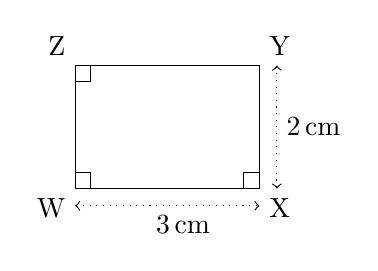
\begin{tikzpicture}[scale=1.1, baseline=(current bounding box.north)]
    \begin{scope}[rotate=0]
        % Draw square
        \draw (0,0) coordinate (W) --
              ++(2.129,0) coordinate (X) --
              ++(0,1.419) coordinate (Y) --
              ++(-2.129,0) coordinate (Z) -- cycle;

        % Right angle markers
        \foreach \p/\q/\r in {Z/W/X,W/X/Y,Y/Z/W,Z/W/X} {
            \pic [draw, -, angle radius=0.2cm] {right angle=\p--\q--\r};
        }

        % Vertex LABELS
        \foreach \p/\l in {W/below left,X/below right,Y/above right,Z/above left} {
            \node[\l] at (\p) {\p};
        }

        % Dotted arrows shifted away from edges
        % Horizontal side (A-B), shifted down
        \draw[<->, dotted]
            ($(W) + (0,-0.2cm)$) -- ($(X) + (0,-0.2cm)$)
            node[midway,below, xshift=2mm] {3\,cm};

        % Vertical side (B-C), shifted right
        \draw[<->, dotted]
            ($(X) + (0.2cm,0)$) -- ($(Y) + (0.2cm,0)$)
            node[midway,right] {2\,cm};
    \end{scope}
\end{tikzpicture}
\end{minipage}%
\hfill
\begin{minipage}{.4\textwidth}
  \begin{align*}
  \text{Area} &= lw \\
  \text{Area} &= 3 \,\text{cm} \times 2 \,\text{cm} \\
  \text{Area} &= 6 \,\text{cm}^2
  \end{align*}
\end{minipage}
\par\vspace{1cm}

\end{document}
